\chapter{Fundamentos y Estado del arte}

%En este capítulo se intentara dar una breve reseña de las investigaciones mas recientes en el campo de las comunicaciones ópticas. 
En este capítulo se presentan las bases y fundamentos de las técnicas desarrolladas y utilizadas en esta tésis. 
Primeramente se da una breve explicación de los conceptos de códigos correctores de errores, continuando con los distintos algoritmos utilizados en la implementación. Luego, se explicará el concepto de espectro ensanchado, una técnica utilizada en comunicaciones pero implementada de un modo poco convencional en este trabajo. Posteriormente se repasarán los aspectos de seguridad a tener en cuenta al utilizar los algoritmos previamente mencionados, los conceptos de niveles de fuerza criptográficas y de cual es el objetivo a alcanzar con respecto a este último tema.

Para finalizar, en la sección de estado del arte se repasarán el estado de las tecnologías y sistemas en uso actualmente, a modo de comparación con el descrito en esta Tesis.

\section{Códigos correctores de errores}

Para trasmitir información digital a través de un medio analógico tal como una fibra óptica, deben convertirse las señales digitales original a señales analógicas.
Toda señal analógica que se transmite o almacen en algún medio físico invariablemente se sufre una degradación, producto de las imperfecciones de los transductores, imperfecciones o limitaciones en la codificación o ruido de diferentes tipos. Esta degradación puede ocurrir en cualquier módulo del sistema, o las interfaces entre los mismos, y generalmente es deseable que el sistema pueda reproducir los datos almacenados o transmitidos con la menor cantidad posible de errores. La diferencia entre la señal transmitida y la recibida se suele modelar como una señal de ruido con una determinada distribución de potencia superpuesta a la señal codificada. Algunos modelos de ruido son muy utilizados, tal como el ruido aditivo gaussiano, utilizado para modelar la interferencia producto de fuentes naturales como ruido térmico o para aproximar fuentes de ruido no-lineales.

Al transmitir datos digitales sobre canales con ruido, aún asumiendo que las etapas moduladoras y demoduladoras son capaces de reproducir los datos fielmente, el mensaje recibido $m_r$ sera distinto del mensaje original $m$, ya que la señal que recibe el demodulador sera una combinación de la señal original del demodulador con el ruido. La diferencia entre la señal recibida $m_r$ y $m$ se denomina error de transmisión. Para aumentar la confiabilidad y reducir el error de transmisión se idearon códigos correctores/detectores de errores, con los que el receptor puede detectar un error y pedir una retransmisión, o bien corregir el error utilizando datos adicionales presentes en la señal. Los métodos de corrección de errores generalmente funcionan reduciendo la entropía de la información transmitida, aumentando la redundancia de la información.

Un método trivial de corrección de errores consiste en utilizar un código de detección de errores como puede ser una suma de verificación, el algoritmo CRC o función de hash \cite{Menezes:1996:HAC:548089}, e iniciar un proceso de retransmisión del segmento o trama de datos afectada. Esté simple método posee la desventaja de ser costoso tanto en ancho de banda utilizado, como en el retraso de la transmisión. En enlaces de muy alta velocidad, las elevadas tasas de retransmisiones hacen a este algoritmo sumamente ineficiente.

Por lo tanto es deseable utilizar un algoritmo que pueda detectar y corregir errores basado solamente en información adicional transmitida, sin utilizar retransmisiones. Esta técnica se denomina \textsl{Forward Error Correction Codes}, o códigos FEC \cite{Moon:05} de los cuales existen diferentes tipos de acuerdo con sus aplicación, performance y parámetros. A continuación, se describen los algoritmos que fueron utilizados en el sistema propuesto en esta Tesis.

\subsection{BCH/Reed Solomon}
Los códigos BCH y Reed-Solomon~\cite{reed1960polynomial} son usados ampliamente en la industria de comunicaciones y almacenamiento masivo ya que la implementación es eficientes desde el punto de vista del radio entre errores corregidos e información de paridad agregada. De echo, Reed-Solomon pertenece a una clase de códigos lineales denominados MDS (\textit{maximum distance separable}) que se consideran óptimos en esta relación. Estos códigos consisten en una representación de los datos basada en grupos algebraicos cíclicos. 
Esta familia de códigos fue introducida en 1959, pero es todavía utilizada en estándares de Ethernet de 10Gbps, 100Gbps y hasta 400Gbps~\cite{liforward} debido a su robustez, bajo retraso y la existencia de algoritmos eficientes para la decodificación en un tiempo fijo.

\subsection{LDPC}
El esquema de corrección de errores LDPC~\cite{gallagerpress} (\textit{Low Density Parity Check}, también conocidos como códigos de Gallager) es un caso notable. Introducido en los años 60, fue olvidado debido a la alta capacidad de procesamiento y memoria requerido por el mismo, ya que para su implementación es necesario utilizar matrices de paridad de un tamaño elevado. Sin embargo, con los modernos avances en hardware informático, éste algoritmo se volvió una opción viable y actualmente es utilizado en sistemas modernos~\cite{brack2007low} debido a su simplicidad y gran capacidad de corrección de errores, en algunos casos muy cercana a la máxima capacidad teórica del canal.
Antes de ahondar en la descripción de este algoritmo debemos aclarar que, a pesar de ser utilizado para ciertos modelos durante la primera fase de la investigación, fue descartado en la versión final por un modelo mas simple y con menos requerimientos de hardware que presenta una desempeño similar desde el punto de vista de corrección de errores.

LDPC es un código que se denomina ``\textit{capacity-approaching}'' esto es, para un canal discreto sin memoria, el ruido del mismo puede ser estar muy cerca del límite teórico de Shannon~\cite{shannon48}.
El algoritmo se basa en un código lineal que utiliza una matriz de paridad $H$ grande y dispersa. Esta matriz tiene la propiedad de que todo codeword $x$ válido cumple con $H*x=0$. 
Existen muchos métodos para construir la matriz de paridad; uno muy utilizado consiste simplemente en generarla aleatoriamente. Otras maneras de generar la matriz son posibles y es un campo de investigación activo actualmente.

% Meter en apendice
%\paragraph{LDPC: Generador de matriz}
%La matriz generadora puede crearse fácilmente si H es de la forma $[D|I]$, simplemente formando la matriz:
%$$G=[I|D']$$
%Donde D' es la transpuesta de la matriz D
%Para la generación de la matriz se opto por utilizar un algoritmo aleatorio y luego aplicando testeos de validación, para lograr una matriz sistemática de rate entero (1/2, 1/3, etc.)
%Para verificar se G genera vectores cuya matriz de paridad es H, puede verificarse que:
%$$ H*G'=0 $$

%Podemos definir la matriz de paridad $H$ como una matriz de paridad que tenga mas de 3 unos por fila y una cantidad similar por columna. Buenos resultados se obtienen a partir de matrices de 200x100.
%Se puede comenzar por una matriz vacía $H = 0$ del tamaño deseado, y ir agregándole unos al azar. Cierto análisis es necesario para garantizar que no se cumplan ciclos y que la cantidad de unos por columna y por fila es la deseada. De esto se encargan los algoritmos llamados evencol y evenrow.

%El generador puede generar matrices de cualquier tamaño, de esta manera:

%$$ ./genMatrix <width> <height> <ones per row>$$

%La matriz se genera en la salida estándar. El formato es el utilizado por la biblioteca boost:ublas [CITA].

%NOTA: La matriz siempre esta compuesta de símbolos en GF(2) (O sea, ceros y unos)

%\paragraph{LDPC: encoder}

%El vector inicial se toma de la entrada estándar (stdin) y el codeword se emite en la salida estándar (stdout). La sintaxis es muy sencilla:

%$$ ./ldpcen <matriz> < in >out $$
%\paragraph{LDPC: decoder}
%Si se invoca este filtro mediante el nombre decodificador, tomara el codeword de la entrada estandard, aplicara el algoritmo de belief-propagation (Hard-decision) y se emite el vector original por la salida estandard:
%La diferencia radica que en nuestro caso, al ser un canal asimetrico no se permite el bit-flip de un valor cero a un valor uno, ya que es imposible que se produzca ese error.
%La linea de comando es la siguiente:

%$$ ./ldpcdec <matriz> <in >out $$

%La conversión codeword->vector es sencilla, ya que al ser un código sistemático solo se necesita eliminar la parte del vector que representa la paridad añadida.

%Se generaron muchas matrices, desde 256x128 hasta matrices muy grandes de 10000x5000, pero el tiempo de decodificación crece enormemente para matrices grandes.

%\paragraph{LDPC: optimización}

%Debido a la naturaleza iterativa del decodificador LDPC, pronto se convirtió en el cuello de botella de la simulación. Para acelerar el sistema, se opto por realizar la siguiente optimización:
%Desde el punto de vista algorítmico, LDPC consta básicamente de varios loops, dentro de los cuales se accede a la matriz de paridad, y a otras matrices que acumulan datos intermedios. Primeramente la implementación fue realizada como mencionamos utilizando boost:ublas, pero luego se comprobó que una implementación utilizando arrays de C era hasta 3 veces mas rápida.
%Luego se procedió a realizar un algoritmo de ``unrolling'' de estos loops, generando código especifico a una matriz dada, sin ningún tipo de loop. Obviamente este código es mucho mas grande, pero la aceleración provista es aun mayor, del orden de 8 veces mas rápido que en implementaciones iniciales.
%La manera de invocar el generador de código es la siguiente:

%$$ ./genLdpcDecoder matriz  > decodeGen.h $$

%El archivo generado decodeGen.h es el decodificador especifico para la matriz dada. Este encabezado de C es luego incluido desde el decodificador ldpcenc.cpp y compilado. Al ser generalmente un archivo de un megabyte para una matriz pequeña de 1024x512, el proceso de compilación el largo y requiere de mucha memoria.
%Por otra parte, no se optimizo el proceso de codificación LDPC, ya que consiste solo de una multiplicación de un vector por una matriz, y es una de las tareas en la que boost:ublas es especialmente eficiente.

%\subsubsection{Viterbi/Convolucional}

\section{CDMA}
\label{espectroensanchado}
La multiplexación por división de código, acceso múltiple por división de código o CDMA (del inglés \textit{Code Division Multiple Access}) es el nombre genérico de varias técnicas de comunicación basadas en el espectro expandido, con el fin de lograr multiplexación o control de acceso al medio. 
Se denomina espectro expandido a la utilización de mayor ancho de banda que el necesario para la transmisión correcta de los datos. Generalmente se logra mediante la combinación de una señal señal de ensanchamiento o de pseudo-ruido, con la señal original, utilizando diferentes métodos.

Los orígenes datan del 1903, cuando Nicola Tesla patentó el concepto de \textit{Frequency hopping} o salto en frecuencia, uno de los métodos de CDMA utilizados actualmente.

Estas técnicas apuntan a agregar las siguientes propiedades en el sistema de comunicaciones:
\begin{enumerate} 
\item Resistencia contra ruido e interferencias: ya que el ruido solo afecta una parte del espectro, ante la presencia de ruido, la mayoría de la señal no se verá afectada, pudiéndose recuperar el resto de la información mediante técnicas de corrección de errores.
\item Resistencia a intercepción: si un atacante no conoce la secuencia que se utilizó para expandir el espectro de la señal original (secuencia generada, por ejemplo, por un generador de números pseudo-aleatorio o PRBS), es dificil diferenciar la señal expandida del ruido.
\item Capacidad de acceso múltiple: varios usuarios pueden transmitir en la misma frecuencia mientras utilicen diferentes códigos.
\end{enumerate} 

Existen varios métodos de CDMA, entre ellos:
\begin{enumerate} 
\item \textit{Direct Sequence Spread Spectrum} (DSSS): Se expande la señal multiplicándola con un código de pseudo-ruido o señal de ensanchamiento, mediante la operación lógica XOR, o mediante desplazamientos de fase. Dicho código es en general modulado a mucha mayor velocidad que la información original. Este método es el utilizado en WiFi y WiMAX, redes 3G de celulares, el sistema GPS, etc.
\item \textit{Frecuency Hopping Spread Spectrum} (FHSS): La señal de ensanchamiento o pseudo-ruido en este caso,  utilizada para variar la frecuencia portadora o canal de la señal original. Este método es utilizado, por ejemplo, en el sistema BlueTooth de comunicación digital. En este caso se utiliza una variación llamada \textit{Adaptive Frequency Hopping}, un método para evitar frecuencias con mucha interferencia.
\item \textit{Time Hopping Spread Spectrum}: En este método, también llamado modulación por posición de pulso, la señal de datos no se transmite todo el tiempo, sino que se divide en pulsos de transmisión, que sufren de un retraso que depende de la señal de ensanchamiento o pseudo-ruido. Actualmente este método no es tan utilizado como los anteriores, aunque se estudiará detenidamente en nuestro caso ya que su implementación sobre una plataforma FPGA (\textit{Field Programmable Gate Array}) con interface óptica es posible sin ningun componente adicional.
\end{enumerate} 


\section{Códigos de generación de pseudo ruido}
\label{PRNGs} 
El código CDMA requiere de una secuencia de pseudo ruido, también denominada pseudoaleatoria, para modular la señal original. Existen muchos algoritmos para generar este tipo de secuencias, dependiendo de las características deseadas.

Ciertas aplicaciones no requieren de una secuencia muy larga, ya que no es necesario cuando el objetivo solo es expandir el espectro de la señal original. Por ejemplo, el protocolo WiFi 802.11b multiplica cada bit con una secuencia de solo 11 bits, denominada secuencia de Barker \cite{mikulka2007cck}.

Si es necesario que la comunicación sea privada, es deseable que la secuencia pseudoaleatoria posea las siguentes características:

\begin{enumerate}
 \item Debe ser solo conocida por las entidades comunicantes.
 \item No se debe repetir la secuencia, para que la misma no se pueda deducir de simple observación.
 \item Ninguna parte de la secuencia debe poder estimarse por una entidad externa a las comunicantes sin conocer los parámetros de generación.
\end{enumerate}

 Esto puede lograrse utilizando un algoritmo denominado generador pseudo-aleatorio o PRBS, que generan la secuencia basadas en un parámetro de inicialización o semilla, siendo capaces de generar un flujo de números aparentemente aleatorios, pero en realidad totalmente determinísticos. Adicionalmente, un generador que cumple con el punto 3) se denomina criptográficamente seguro, ya que es apto para su uso en criptografía.
 
Es necesario que los nodos que participen de toda comunicación privada puedan generar exactamente la misma secuencia, por lo que deberán compartir el parámetro de generación, comunmente denominado \textit{semilla}.

Existen muchos métodos o algoritmos para generar flujos de números pseudo-aleatorios. Un parámetro importante, nombrado en el punto 2) de la lista al principio del capítulo, es la cantidad de bits que es capaz de emitir antes que se repita la secuencia o período. Este parámetro es denominado el período del generador, y en aplicaciones criptográficas es deseable que sea lo mas grande posible. 

Pero el echo de tener un período largo no es suficiente para que el generador pseudoaleatorio pueda ser utilizado en aplicaciones criptográficas. Podemos citar el caso del algoritmo denominado Mersenne-twister \cite{matsumoto1998mersenne}, cuya aplicación mas popular tiene un período de $2^{19937}-1$, pero sin embargo existen métodos para predecir la secuencia sin conocer la semilla \cite{argyros2012forgot}, por lo que no es apto para aplicaciones seguras.
Otra características deseable en un generador PRBS son su baja complejidad, bajo consumo de recursos y alta velocidad de generación. Un generador PRBS muy popular utilizado ampliamente en implementaciones de software es el denominado generador congruencial lineal \cite{park1988random}, un algoritmo extremadamente simple que solo precisa de dos operaciones: una multiplicación y una suma, siendo muy utilizado en aplicaciones de estadística y software.

\subsection{Generadores criptográficamente seguros}

Estos ejemplos mencionados en la sección anterior carecen de una característica fundamental requerida en nuestro sistema: Que no se puedan predecir. Esta simple característica no es en realidad trivial ya que existen técnicas \cite{argyros2012forgot} para inferir datos acerca del generador PRBS, lo que supondría la falla total en la seguridad de un sistema basado en dicho generador. Los algoritmos que no sufren de este problema son llamados generadores PRBS criptográficamente seguros o por las siglas en inglés, CS-PRNG. Como ejemplo podemos nombrar a los generadores del tipo shrinking~\cite{coppersmith1994shrinking}.
Constantemente surgen nuevos ataques a generadores ampliamente utilizados, tales como el generador utilizado por el algoritmo RC4~\cite{vaudenay2007passive}, por lo que es imprescindible estar actualizado en los avances de investigación criptográfica para diseñar un sistema seguro. En el caso de RC4, el mismo creador (Ron Rivest) ha desarrollado recientemente un reemplazo corrigiendo varias vulnerabilidades y manteniendo las características deseables denominado Spritz~\cite{RS14}. Los generadores pseudoaleatorios suelen ser costosos computacionalmente , una de las razones por la cual las transmisiones de muy alta velocidad no suelen estar encriptadas, aunque avances en hardware con aceleradores específicos para criptografía \cite{firasta2008intel} están logrando que la implementación de enlaces criptográficos sea cada vez mas masiva.

\section{Seguridad}
\label{Seguridad}

Se propone utilizar un sistema de espectro expandido con el objetivo principal de lograr la privacidad del canal al nivel físico en el sistema de comunicaciones óptico y acústico.
Se fijaron los siguientes parámetros de seguridad:

\begin{itemize}
 \item El sistema debe proveer confidencialidad, integridad y autenticidad de los datos.
 \item El sistema debe ser seguro sin importar la cantidad de clientes existentes o la naturaleza de los datos que se transmiten.
 \item Un atacante no debe poder identificar los datos de un cliente, aunque controle todos los demás nodos de la red. O sea, el sistema debe garantizar privacidad ante un ataque coordinado donde la mayoría de los nodos de la red son maliciosos. Esto evita el uso de ciertos algoritmos \cite{gold1967optimal} donde al conocer la secuencia de la mayoría de los nodos, se puede inferir la secuencia de cualquier otro nodo en particular.
\end{itemize}

Con estos parámetros se busco el algoritmo CDMA adecuado. Si bien la implementación en un sistema acústico no presenta grandes limitaciones en la técnica utilizada debido a los bajos recursos computacionales necesarios, las características de un sistema óptico de alta velocidad hacen muy complejo el hardware requerido para lograr CDMA o Frequency-Hopping. Sin embargo implementar time-hopping no presenta costo ni dificultad adicional, por lo que fue el seleccionado para la implementación del aspecto de seguridad del sistema.

Como se explico anteriormente, el algoritmo de time-hopping consiste en dividir el tiempo en segmentos denominados frames, compuestos de \textit{slots} o casilleros, y modular el slot asignado a cada transmisión por medio del generador PRBS, de esta manera puede verse como la señal efectua saltos o ``hops'' en el tiempo a medida que es transmitida en diferentes slots. Varios algoritmos para la asignación del slot fueron analizados. 

Una propiedad deseable es que los códigos generadores de cada canal sean ortogonales entre sí, es decir que si bien los códigos generados son pseudo-aleatorios, la salida de dos o más generadores nunca coincide al mismo tiempo, para así evitar colisiones entre los canales donde se intenta transmitir en el mismo slot al mismo tiempo, invalidando la transmisión para todos los clientes que colisionan.
Sin embargo para lograr esta característica es necesario compartir algún tipo de información entre todos los clientes, lo que debilita la seguridad del sistema. Por ejemplo, códigos existentes llamados Gold-codes~\cite{gold1967optimal} permiten la generación de múltiples secuencias con baja correlación cruzada, utilizadas para coordinar dispositivos que comparten el medio, ya que garantizan la carencia de colisiones. Pero desde el punto de vista de la seguridad, este código es trivialmente derrotado. Por ejemplo, en un esquema donde un atacante controla todos los canales menos uno, el atacante podría simplemente dejar de transmitir y revelar la secuencia utilizada por la víctima, que forzosamente estará utilizando el canal restante.

Por este motivo se decidió utilizar una codificación trivial: seleccionar el slot de acuerdo a una secuencia criptográficamente segura estándar, totalmente independiente de los otros canales. Este simple método causará colisiones entre los slots de transmisión, que aumentan exponencialmente con el número de clientes activos. Sin embargo, estas colisiones pueden ser corregidas mediante codificación adicional, y se logró una utilización de canal muy cercana al máximo teórico como se demuestra en la próxima sección. De echo, es en esta codificación adicional donde reside el principal aporte de esta Tesis.

\subsection{Consideraciones de seguridad y fuerza de cifrado}\label{Seguridad-fuerza}
%% extraido de dline-pub.tex
Existen varios aspectos de seguridad en un canal de comunicaciones: autenticación, confiabilidad, confidencialidad e integridad.
El esquema presentado en esta Tesis utiliza la técnica de CDMA para proveer confidencialidad, confiabilidad e integridad entre dos o mas partes, y es equivalente a un esquema de clave simétrica donde la clave compartida es utilizada para inicializar la semilla del algoritmo generador de PRBS. Aspectos adicionales, tales como la autenticación, pueden ser implementados luego utilizando protocolos de alto nivel \cite{krawczyk2001order}.
El sistema propuesto fue específicamente diseñado tomando en consideración los ataques del tipo mencionados en Ref. \cite{Shake:05}.
Como la seguridad del sistema es dependiente de su algoritmo generador de PRBS, se debe poner especial cuidado en la selección e implementación del mismo, que debe ser un algoritmo generador de números aleatorios para usos en criptografía, es decir criptográficamente seguro (CS-PRBS). Existen muchos algoritmos que cumplen con estos requisitos, y el CS-PRBS propuesto en esta Tesis es el llamado self-shrinking generator~\cite{Meier:94}, pero puede utilizarse cualquier otro e incluso usar diferentes algoritmos para cada cliente, con la condición que dos clientes que deseen comunicarse deben utilizar el mismo algoritmo con los mismos parámetros y claves.
Como es en el caso de otros algoritmos de clave simétrica, la clave secreta debe distribuirse previamente utilizando un canal seguro.

Existe una vulnerabilidad adicional inherente a sistemas ópticos dispuestos como una red en estrella como el propuesto en este trabajo: los algoritmos de CDMA dependen de la interferencia para ofrecer confidencialidad. Sin embargo, en un sistema óptico con topología en estrella hay secciones donde existe poca o ninguna interferencia. Un ejemplo es el segmento próximo a la salida de un transmisor, donde la señal de entrada esta atenuada y por lo tanto es inferior a la señal de salida, que puede diferenciarse con respecto al ruido de las demás transmisiones.   
Esta y otras vulnerabilidades fueron subsanadas en cuenta en el diseño final mediante ajustes en la codificación.
%Para contrarrestar estas situaciones los símbolos productos de la minimización del peso de Hamming fueron normalizados con respecto a un dígito normal, por lo que aún si un atacante pudiera escuchar y discriminar cada uno de los bits de salida, no podría decodificarlos ni inferir información alguna acerca de los bits transmitidos.
%Como los distintos clientes emitiendo dentro de una trama se puede superponer, el atacante observara un símbolo con un HW entre 1 y W$\times$K, pero no es posible reconstruir el orden correcto de los bits sin la semilla del algoritmo generador de PRNG.

Otra característica del algoritmo de encriptación es que no modifica el peso de Hamming del flujo de bits. Muchos algoritmos de cifrado se basan en la operación de XOR (El caso del algoritmo RC4), o bien una combinación de sustituir/transponer los datos antes de la transmisión (El caso de algoritmos AES y DES), o transformaciones mas complejas (Caso RSA o algoritmos de curvas elípticas), ver Ref.~\cite{Menezes:1996:HAC:548089}.
Sin embargo, todas estas técnicas necesariamente modifican el peso de Hamming de cada símbolo. % en una manera que no es óptima para el esquema propuesto combinado de CDMA/filtros de Bloom ya que incrementa la interferencia inter-símbolo.
Como el algoritmo propuesto se basa en CDMA del tipo time-hopping, efectivamente se encriptan los símbolos de entrada mientras que mantiene inalterado el peso de Hammings en los datos de salida, una propiedad util para ciertas codificaciones utilizadas posteriormente. % se refleja menor error y en una mayor utilización del ancho de banda disponible como se muestra en la Fig.~\ref{fig_use}.

\begin{figure}[t]
  \centering
  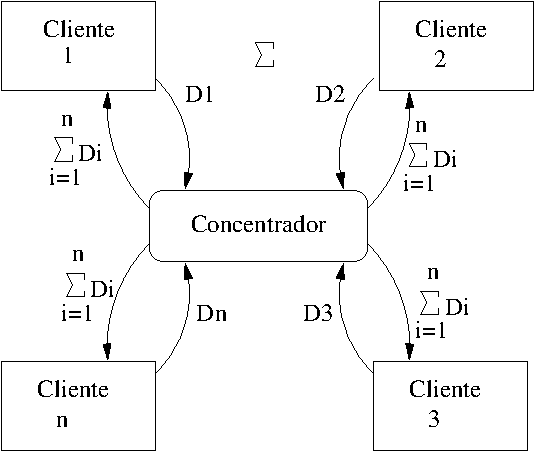
\includegraphics[width=0.6 \textwidth]{graphs/concentrador} 
  \caption{Esquema del concentrador central donde se observa que el flujo de datos de retorno es siempre la sumatoria de todos los datos de entrada.}
%  \caption{Utilizacion del canal de 10 Gbps. Cada uno de los clientes (variando de 123 a 158) transmitieron 1 Gbit de datos. Notar la mejora en la utilización del ancho de banda comparada con~\cite{ortega11}.}
  \label{fig_use}
\end{figure}

Podria discutirse que el sistema es similar al esquema TDMA (\textit{Time Division Multiple Access}) donde también se divide el tiempo en tramas y slots. Pero en contraste con TDMA, en el esquema propuesto el atacante necesita interceptar cada una de las fibras ópticas para identificar cada usuario ya que no es posible identificar exactamente el slot de transmisión luego de pasar por el concentrador central. Aun si el atacante puede identificar los datos, no podrá descifrarlos sin poseer la clave correcta al estar los datos desordenados por el time-hopping y normalizado el peso de Hamming.

\section{Estado del Arte}

A continuación se repasarán las tecnologías disponibles actualmente para realizar encriptación sobre fibra óptica a altas velocidades y otros tipos de redes con esquemas similares al propuesto:

\subsection{Criptografía clásica}
Las comunicaciones ópticas pueden utilizar sin problemas algoritmos de criptografía clásicos tales como encriptación de clave simétrica y asimétrica. La única dificultad consiste en que el procesamiento de datos debe ser lo suficientemente rápido para poder aplicarse al enlace de alta velocidad, lo que conlleva altos costos y procesadores con un alto consumo de energía, aunque la velocidad máxima de procesamiento puede reducirse arbitrariamente utilizando procesamiento en paralelo \cite{liforward}.

Actualmente, un dispositivo muy utilizado capaz de realizar criptografía a alta velocidad sobre fibra óptica es la FPGA, que con la correcta paralelización del procesamiento de datos, puede alcanzar la velocidad máxima permitida por sus transceptores (por ejemplo, 400 Gbps~\cite{Algotronix}).

\subsection{Criptografía puramente óptica}
\label{optocry}
Un campo de investigación activo en la actualidad es el de la criptografía puramente óptica. La eliminación de las etapas electrónicas y la conversión electro-óptica de los datos para su procesamiento tiene muchas ventajas, principalmente en velocidad y potencia consumida por el sistema.
La dificultad principal en este método consiste en lograr una fuerza de cifrado adecuada, y la implementación de los algoritmos necesarios solamente utilizando componentes ópticos. Podemos citar algunos resultados publicados tales como los avances en la creación de compuertas lógicas puramente ópticas \cite{jung2008demonstration}, o la utilización de señales caóticas para transmisión~\cite{liu2002synchronized}.
Debido a su novedad, no existen implementaciones prácticas de esta tecnología utilizada en la industria al momento de la escritura de esta Tesis.

%High speed all-optical encryption and decryption using quantum dot semiconductor optical amplifiers 	http://www.tandfonline.com/doi/abs/10.1080/09500340.2013.856486#.VNHcKPtue00

\subsection{Encriptación cuántica}

\begin{figure}[t]
  \centering
  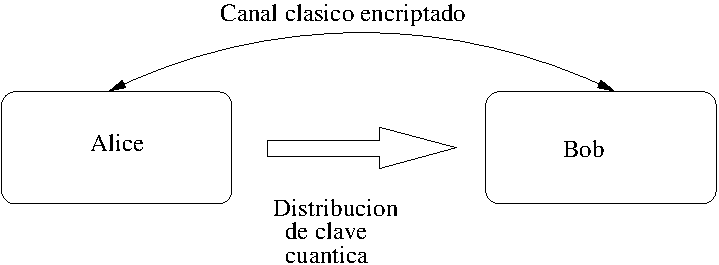
\includegraphics[width=0.7 \textwidth]{graphs/quantum} 
  \caption{Esquema típico del método de distribución cuántica de claves. Al utilizar detectores de mayor complejidad, el canal cuántico posee generalmente menor ancho de banda que el clásico, pero es suficiente para la transmisión segura del material de clave.}
  \label{fig_quant}
\end{figure}


\label{quantcry}
Una solución muy interesante a varios problemas criptográficos son las llamadas técnicas de criptografía cuántica, donde se aprovechan fenómenos de mecánica cuántica para lograr seguridad en las comunicaciones digitales.
En estos sistemas, se codifica la información en estados cuánticos o \textit{qubits}, en lugar de los bits comúnmente utilizados para codificar datos en comunicaciones clásicas, que utilizan efectos físicos clásicos. Generalmente, se utilizan fotones para generar y medir dichos estados cuánticos, por lo que el medio de transmisión suele ser la fibra óptica, aunque es también es posible utilizar el aire como medio \cite{alleaume2004experimental}.
Uno de los problemas criptográficos resueltos utilizando mecánica cuántica es el de la distribución de claves. Algoritmos maduros de distribución cuántica de claves (Quantum key distribution~\cite{bb84}) actualmente son utilizados por la industria y cuentan con implementaciones comerciales e instalaciones a nivel metropolitano~\cite{sasaki2011field}. 

Dependiendo de la propiedad física aprovechada, los sistemas cuánticos pueden dividirse en dos categorías:
\begin{enumerate}
 \item Sistemas basados en mediciones de variables físicas, en los que a diferencia de lo que ocurren en la física clásica, la medición de un parámetro físico afecta el estado cántico de alguna manera. Esto se conoce como indeterminación cúantica, y es utilizado para detectar cualquier interceptación de los datos, que necesariamente deberá realizar una medición sobre los mismos. Por ejemplo, un parámetro comúnmente seleccionado para codificar la información es la polarización del fotón \cite{muller1993experimental}.
 \item Sistemas basados en el entrelazamiento cuántico (\textit{quantum entanglement}) \cite{jennewein2000quantum}, donde los estados cuánticos de dos o más elementos quedan unidos de forma que deben ser descritos mediante un estado cuántico combinado, y no como objetos individuales. Esto causa que la medición en uno de los objetos afectará a los otros, y de esta manera puede detectarse cualquier interceptación.
\end{enumerate}

La seguridad de ambos métodos consiste en detectar una posible interceptación, en lugar de prevenir el acceso a los datos.

Generalmente se utilizan varios canales sobre una fibra óptica, unos llamados ``canales cuánticos'' utilizados solamente para la distribución de claves, y otros ``canales clásicos'' donde se utiliza criptografía clásica (ver esquema en la figura~\ref{fig_quant}).

Vale mencionar que la distribución segura de claves también puede realizarse en un canal clásico por medio de algoritmos matemáticos tales como Diffie-Hellman~\cite{diffie1976new} o bien la utilización de esquemas de clave pública.

Resumiendo, la seguridad de sistemas de criptografía cuántica se basa en las bases de la mecánica cuántica, en contraste con sistemas de criptografía tradicional que se basan en la complejidad computacional de ciertas funciones matemáticas \cite{kohnfelder1978towards}. Sin embargo, vulnerabilidades y fallas en la implementación afectan la seguridad de ambos tipos de sistemas de la misma manera~\cite{lydersen2010hacking}.


\subsection{Corrección de errores de canales asimétricos}

Una sección importante de esta Tesis es la descripción de una técnica de corrección de errores de canales asimétricos basada en el algoritmo de filtros de Bloom (ver~\ref{zbloom}). 
Se denominan códigos de corrección de errores asimétricos o unidireccionales, a todo código de corrección especializado en canales de comunicaciones cuya probabilidad de error no se aplica simétricamente a todos los símbolos. Un caso sencillo es por ejemplo el canal Z, un canal binario (símbolos uno y cero) pero cuyos errores solo pueden afectar un símbolo, por ejemplo esta descripción puede aplicarse a un sistema donde al transmitir el símbolo cero, es posible que un error suceda y sea recibido incorrectamente como un uno, pero lo contrario no es posible. En la figura \ref{fig:Gal} se observa el diagrama de probabilidades del canal binario asimétrico o canal Z. En la sección \ref{canalZ} se desarrolla el límite de capacidad del canal Z.

 Al poder corregir errores sin discriminar el símbolo, puede decirse que todo código de corrección simétrico es también un código de corrección asimétrico.

Recientemente surgió interés en campo de corrección de errores de canales asimétricos, debido a la utilidad de estos algoritmos en sistemas de almacenamiento digitales\cite{tanakamaru201195}. Sin embargo, el número de artículos publicados acerca del tema sigue siendo muy reducido en comparación con las investigaciones de códigos de corrección para canales convencionales. Como ejemplo de un códigos unidireccionales podemos citar los códigos de Berger \cite{berger1961note} y códigos de Gallager o LDPC unidireccionales \cite{neri2008gallager}.

\subsection{Sistemas de comunicaciones ópticas}

Existen muchos esquemas tales como EPON~\cite{kramer2002ethernet} y sus derivados APON/BPON, utilizados por millones de usuarios en la actualidad \cite{chanclou2013france}.
Sin embargo, el sistema que mas se aproxima al descrito en esta Tesis es el SPON (Secure Passive Optical Network). Existen muchos sistemas comerciales que proveen SPONs actualmente. En estos sistemas, se agrega una capa de seguridad clásica por sobre un protocolo de comunicaciones  pre-existente como G-PON (\textit{Gigabit Passive Optical Network}).

Sistemas académicos se basan en encriptación puramente óptica tal como la descrita en \ref{optocry} (Ver~\cite{cincotti2009secure}). Algunas implementaciones proveen la misma funcionalidad que el sistema descrito en esta Tesis, tale como~\cite{nadarajah2006implementation} aunque se diferencian en tipo de CDMA utilizado y la topología de la red óptica.

\subsection{Encriptación de comunicaciones acústicas}

En general, los sistemas de seguridad aplicadas a comunicaciones acústicas han sido siempre en forma de capas adicionales de alto nivel funcionando por sobre las capas físicas. Debido al poco ancho de banda disponible en el espectro de audio (menos de 100 Khz), las comunicaciones acústicas tienen un ancho de banda reducido y es muy conveniente utilizar software para todo proceso criptográfico. Sin embargo existe ejemplos de modems acústicos comerciales capaces de encriptar su enlace \cite{arcelect}, y recientemente se han publicado esquemas en los que también se utiliza la propiedad caótica de la sensibilidad a condiciones iniciales para crear un sistema criptográfico, esta vez sobre canales acústicos \cite{gnanajeyaraman2009audio}.
